\documentclass[letterpaper,12pt]{article}
\pagestyle{empty}

\pdfpagewidth 8.5in
\pdfpageheight 11in

\hoffset = 0pt
\oddsidemargin = 0pt
\marginparwidth = 0pt

\voffset = 0pt
\topmargin = 0pt
\headheight = 0pt
\headsep = 12pt

\textwidth = 6.5in
\textheight = 9in
\footskip = 0pt

\usepackage{amsmath}
\usepackage{amssymb}
\usepackage{hyperref}
\usepackage{graphicx}

\author{Erik Keever}
\title{Imogen User's Manual}

\begin{document} 

\maketitle

\section{Setup}

This section will guide you through the Imogen acquisition and setup process.

The setup process consists in making sure that you have the proper libraries
available and informing Imogen of where they are through the Make.config file
in the top level directory. The template Make.config.default should be copied
to Make.config and then setup per instructions below.

\subsection{Download}

Imogen lives online at \url{https://github.com/imogenproject/gpuImogen}

To download it into directory \textit{./gpuimogen} from the public repo,

\textit{ git clone https://github.com/imogenproject/gpuImogen.git ./gpuimogen }

\subsection{Matlab}

Imogen runs in Matlab and so obviously Matlab is a prerequisite to have. A standard
Matlab installation will have everything you need - the parallel computing toolkit
is not needed.

The \textit{MATLAB\_DIR} variable in Make.config must be set to the root of
the Matlab installation (e.g. /opt/Matlab/R2013b). Running Imogen in a different
Matlab version than used here to compile the binary modules is less likely than
might be imagined to cause problems.

\subsection{MPI}

MPI, even if parallel processing is not used, must be available (Imogen still
uses MPI to check that it is running serially), including development headers
to compile the Matlab mex files.

In Make.config, \textit{MPI\_DIR} must refer to the directory containing the include/ folder
that holds the mpi.h file, i.e. the --prefix specified when MPI was installed.

\subsection{Parallel Gateway}

Imogen uses the Parallel Gateway (PGW) library as a go-between with MPI.

Make.config's \textit{PGW\_DIR} variable must be set to the install directory
containing PGW.

\subsection{CUDA}

Imogen's GPU routines are written in CUDA and access to cuda 4.0 or later
libraries is required. The runtime alone isn't sufficient, the SDK is
needed to provide the headers.

Once it is installed set \textit{CUDA\_DIR} to the install location.

Other variables to be set are
\begin{itemize}
\item \textit{CUDA\_LDIR} - either 'lib' on 32bit or 'lib64' on 64bit machines
\item \textit{NVARCH} - \textit{compute\_20} for Fermi, \textit{compute\_30} for Kepler
\item \textit{NVCODE} - \textit{sm\_20} for Fermi, \textit{sm\_30} for Kepler
\end{itemize}

NVARCH and NVCODE are further explained by the nvcc manual page.

\subsection{Compiling}

Once all the above variables are set, run \textit{make} in both the mpi/ and gpuclass/
directories. Both build in parallel so feel free to use -j. 

\subsection{Filesystem}

Imogen will open/create the directory ~/Results. It is not required that this
be a shared filesystem.

\subsection{Cluster access}

Imogen invokes itself in parallel with the './imogen cluster ...' format.

This takes place on lines 95 to 124 of the run/imogen file. Before running
in parallel on a cluster it would be a good idea to examine this section since
it will almost certainly need to be amended, if only to set the package
names to their local values.

\subsection{Troubleshooting}

It is very important that PGW, MPI and the CUDA modules all be compiled
using the same compiler. PGW in particular is insistent about the version
of libfortran it accesses.

Unfortunately this is growing progressively more difficult as CUDA requires
newer GCCs and Mathworks' MEX compiler-wrapper lags.

If Imogen fails because Matlab complains about being unable to resolve an MPI
symbol, the problem is that Matlab defaults to lazy symbol resolution when
loading dynamic libraries and apparently something about the MPI lib trips
up on this. The solution:
\begin{itemize} \item LD\_PRELOAD="\$MPIDIR/lib/libmpi.so"
\end{itemize}
Putting this in your .bashrc (or as sysadmin, in the system's /etc/profile.d) will
make it go away permanently.

\section{Invocation}

Imogen is run through the script run/imogen

There are three separate general types of run, all of which end up doing "matlab -r":
\begin{itemize}
\item serial - One process uses ones GPU; 'imogen' calls Matlab.
\item parallel - N processes select N GPUs; 'imogen' calls mpirun calls Matlab
\item cluster - N processes on M nodes; 'imogen' writes a script for qsub that calls Matlab
\end{itemize}

Serial and parallel are for small size simulations that work on a single SMP system,
while the cluster option uses qsub to fire jobs onto large systems.

The invocation syntaxes (also available through ./imogen -help) is as follows:
\begin{itemize}
\item ./imogen serial runfile.m [stream\# [GPU\#]];
\item ./imogen runfile.m; A shortcut that assumes serial, stream 0 and GPU 0.
\item ./imogen parallel runfile.m [stream\#] [NP]
\end{itemize}

\section{Selftest}

\textbf{This is not yet complete -- Erik}

Imogen includes a comprehensive full-simulation test, the simulation
\textit{run\_FullTestSuite.m}. This ``simulation'' will run dozens of test cases
for which an exact solution (or reasonable facimile thereof) is available
and determine whether Imogen is going them right and, where analytic answers
are available, provide convergence orders.

Note that there are a lot of tests to run, and this test falls under the "go have
lunch then check back" class.

\section{Physics solved by the Imogen simulation engine}

\subsection{CFD}

At its core Imogen solves the Euler equations, written here in conservative form:
\begin{align*}
\frac{\partial \rho}{\partial t} &= -\frac{\partial}{\partial x_i} \rho v_i \\
\frac{\partial (\rho v_i)}{\partial t} &= -\frac{\partial}{\partial x_j} (T_{ij} + \mathbb{I} P) \\
\frac{\partial E}{\partial t} &= -\frac{\partial}{\partial x_i} v_i (E + P)
\end{align*}
with mass density $\rho$, fluid bulk velocity $v_i$, momentum stress tensor
$T_{ij} = \rho v_i v_j$, identity tensor $\mathbb{I}$, scalar thermal pressure $P$,
and total energy density $E = \frac{1}{2} \rho v^2 + \epsilon$.

These are closed by the equation of state $P(\epsilon)$. Imogen implements the
adiabatic ideal gas equation of state, $P = (\gamma-1)\epsilon$ for $\gamma > 1$
(physical gas values are $1 < \gamma \le 5/3$).

With the assumption of a gamma law, the energy flux is written into the
code as $v_i \times (\frac{1}{2} \rho v^2 + \frac{\gamma}{\gamma-1}P)$ with $P$ calculated
before fluxing.

\subsubsection{Operator splitting}

Imogen uses a dimensionally split flux solving scheme. Assuming a splittable Hamiltonian
exists in the form
\[\mathbf{H} = \mathbf{E} + \mathbf{F} + \mathbf{G}\]
where in our case, $E$, $F$, and $G$ represent the fluid fluxes in 3 non-degenerate
directions (normally taken as 3 orthogonal directions in a curvilinear coordinate
system: Here, fluxes in the x, y, and z directions), an approximate scheme of the form
\[e^{\epsilon \mathbf{H}} = e^{\epsilon \mathbf{E}} e^{\epsilon \mathbf{F}}
e^{\epsilon \mathbf{G}} + \mathbb{O}(\epsilon^2) \]
always exists, and the reader may easily verify that the local error associated with
doing this with two operators equals their commutator times $\epsilon^2$.

Strang [reference!] showed that by performing such a first order step, then
applying the same operators in exactly reversed order, will cancel all the first-order
errors. This Strang splitting provides an easy way of constructing second spatial order
solvers.

Denoting the operators that solve the inviscid flux equations in the three directions as
$\mathbf{X}$, $\mathbf{Y}$ and $\mathbf{Z}$, there are 6 ways to order them which are the
elements of the permutation group of $\{ \mathbf{X}, \mathbf{Y}, \mathbf{Z} \}$.
In a two-dimensional simulation, there are only two orderings ($XYYX$ and $YXXY$).

Imogen cycles through them iteration to iteration, the idea being that this will average
away (or at least partly so) any systematic errors associated with a given ordering.

There are additional operators associated with MHD (magnetic fluxing operators), non-inertial
frames, radiation, and scalar potental fields (fixed potentials, point objects or
self-gravitation).

\textbf{The MHD algorithm has major problems with low-beta plasma and seems to be
subtly broken at present.}

\subsection{MHD}

Imogen can evolve magnetic fields in the limit of Ideal MHD where the Euler equations
become
\begin{align*}
\frac{\partial \rho}{\partial t} &= -\frac{\partial}{\partial x_i} \rho v_i \\
\frac{\partial (\rho v_i)}{\partial t} &= -\frac{\partial}{\partial x_j} (T_{ij} + \mathbb{I}(P+B^2/2) \\
\frac{\partial E}{\partial t} &= -\frac{\partial}{\partial x_i} v_i (E + P) - B_i (v_j B_j) \\
\frac{\partial B_i}{\partial t} &= \frac{\partial}{\partial x_i} (v_i B_j - B_i v_j)
\end{align*}
now with the stress tensor $T_{ij} = \rho v_i v_j - B_i B_j$ and under the requirement
$\nabla \mathbf{B} = 0$.

There is no computational requirement that the \textbf{B} field be initialized this way,
however Imogen solves no advection equation for $\mathbf{B}$-charge and any divergence
introduced will simply stay there.

\subsection{Frame rotation}

In many cases a simulation is desired of an object that exhibits coherent rotation at
high speeds.

Imogen has the Eulerian explicit CFL constraint is set by
\[ dt < dx (|v_i| + c_s) \]
and so if $v_i$ can be significantly reduced by setting the grid to co-rotate with a flow,
the timestep can be significantly increased for advection-dominated flows.

The non-inertial sourcing operator introduces its own errors and it is up to the user to
determine the point at which the change is worth it.

Imogen checks for a rotating frame at simulation initialization and performs the
transformation to the noninertial frame for you - simulations should be initialized
in the lab inertial frame.

\subsection{Radiation}

Imogen can solve optically thin radiation with power law cooling,

(power law lambda)

Programming in different cooling laws is extremely simple as a test by making additional
entries to the experiment/Radiation.m file, templatted after the thin power law radiation
one. Of course, don't expect them to be as fast as the GPU accelerated routines.

While the power law cooling is reliable enough in and of itself, it has exhibited a
remarkable ability to derange Imogen's fluid solver routines. None of them has exhibited
the ability to handle an extremely slowly-moving radiating shock front (i.e. the motion
associated with the finite accuracy of the simulation) without some measure of oscillatory
density error at the adiabatic jump.

(Post pics of evil radiative shocks here)

\subsection{Gravity}

\subsubsection{Point gravity}

Imogen allows the addition of massive points to the fluid simulation which obey Newton's
laws. Both point-point and point-fluid gravitational force are computed.

These points, ``compact objects'' as Imogen calls them, are used as standins for stars
or planets which cannot be resolved at reasonably available levels of resolution.

Far away from the object, they behave as point masses. Within a distance defined as
its 'radius', matter is considered as having been accreted. Each step, the mass and
linear and angular momentum in cells whose center is within r of a compact mass
are added to the compact object and replaced with grid's vaccuum values instead.

NOTE: This is not the desired behavior in some cases - e.g. a planet would require a surface
pressure, not a surface vaccuum, in order to be embedded in the disk.

\textbf{Point does not feel fluid gravity presently.}

\subsubsection{Self gravity}

This is basically dead for now, especially in parallel.

The serial solver could easily enough be resurrected but there's no way I'm going
to have time to setup a parallel Poisson solver, let alone shovel it onto the GPU.

\section{Physics solvers in the initializers}

Many fluid and physics subproblems come up when writing initial condition generators
for Imogen. Some of these have convenient self-contained solvers available within
Imogen.

The available units include:
\begin{itemize}
\item \begin{tt}J = HDJumpSolver(Mach, $\gamma$, $\theta$)\end{tt}: Returns a structure $J$ describing the
only physical shock solution to a hydrodynamic shock of strength $Mach$ in a fluid of
adiabatic index $\gamma$ and preshock shock-normal flow inclination $\theta$ (in degrees).
\item \begin{tt}J = MHDJumpSolver(Mach, Alfven Mach, $\gamma$, $\theta$)\end{tt}: Solves the MHD jump
equations for the slowest shock permitted.
\item \begin{tt}F = fim(X, @f(X))\end{tt}: Short for Fourier Integral Method, calculates the integral of
anonymous function f on the presumed regularly spaced points $X$ by calculating a polynomial
that renders $f$ 3 times continuous at the endpoints, integrating the polynomial directly
and the residual by Fourier transform.
\item \begin{tt}The ICM\end{tt}: \begin{tt}icm.m\end{tt} is currently very much a prototype and not ready for normal use.
It is short for Integral Constraints Method.
\item \begin{tt}t = pade(c\_n, a, b, x)\end{tt}: Given a polynomial $\sum_n c_n x^n$, calculates the (a,b)
Pade approximant P(a)/Q(b) of the polynomial and evaluates it at x, for any $a+b \le 6$.
\item RadiatingFlowSolver class: Solves the equations of a power-law-radiating hydrodynamic
or magnetohydrodynamic flow. It initializes itself using the 4th (MHD) or 6th (HD) order power
series solution of the flow and then integrates using a 6th order implicit LMM, restarting with
reduced step size when it encounters sharp flow features (knees).
\item Linear wave eigenvectors: The function eigenvectorEntropy, eigenvectorAlfven, eigenvectorSonic,
eigenevectorMA(rho, csq, v, b, k, wavetype) return the linear wave eigenvectors associated with the
flows with the given uniform density, thermal acoustic soundspeed, velocity, magnetic field and wavevector.
Alfven and sonic waves have wavetype +1 for a wave which advances towards $\mathbf{k}$ and -1 for
against $\mathbf{k}$. The MA wavetype can have either sign, with magnitude 2 for a fast MS
wave and magnitude 1 for a slow MS wave. If a nonzero B is passed to a sonic wave, it will invoke the
fast MS solver (as the fast wave is the one connected with the nonmagnetized sonic wave).
\item The bow shock problem, in two-dimensional testing of a source with outflow, has acquired a routine
analyticalOutflow() which solves the exact adiabatic expansion of a $\gamma=5/3$ gas away from a cylinder
with the inner boundary condition of $v_{radial} = v_0$ at $r=r_0$.
\end{itemize}

\section{Programming Experiments}

\subsection{Common parameters of all experiments}

All experiment initializers should inherit from the \begin{tt}Initializer\end{tt} class
and share its not inconsiderable breadth of parameters. Among the more important 
names are
\begin{itemize}
\item \begin{tt}cfl\end{tt} coefficient by which the CFL-limit timestep is scaled. \textbf{WARNING
IMOGEN DOES NOT SANITY CHECK THIS}
\item \begin{tt}gamma\end{tt} - The adiabatic index of the fluid
\item \begin{tt}grid\end{tt} - The [nx ny nz] grid resolution of the \textit{global} domain. This
should normally be set when creating the initializer and not messed with again.
\item \begin{tt}iterMax\end{tt} - the maximum number of timesteps to take
\item \begin{tt}useInSituAnalysis\end{tt} - If nonzero, Imogen uses the given in-situ analysis tool
\item \begin{tt}inSituHandle\end{tt} - @AnalyzerClass which must meet the requirements of an
in-situ analyzer (see REF)
\item \begin{tt}stepsPerInSitu\end{tt} - Number of timesteps between calls to the analyzer
\item \begin{tt}frameRotateOmega\end{tt} - If nonzero, Imogen places the simulation into a rotating
frame and applies appropriate source terms. \textbf{Simulation is still initialized in lab frame}
\item \begin{tt}frameRotateCenter\end{tt} - If frame is rotating, this is the center (\textbf{in cells})
about which the frame rotates on the $(x,y)$ plane.
\end{itemize}

\subsection{How to setup frame rotation}

To turn on the rotating frame during start, simply set a nonzero value for the \begin{tt}frameRotateOmega\end{tt}
parameter, and assign a 2-element array $\left[x_0, y_0\right]$ to \begin{tt}frameRotateCenter\end{tt}
and Imogen will automatically transform the fluid momentum field into the noninertial frame at start.

Caution: $x_0$ and $y_0$ need to be in cell coordinates... yes it's dumb.

The rotation rate can be altered during simulation time using 
\begin{tt}
alterFrameRotation(run, mass,\newline
ener, mom, newOmega)
\end{tt}
in the user's in-situ analysis function. This has no physical effect (outside truncation error)
and will not e.g. generate the Euler term, it simply alters the rate at which the grid traverses
the fluid in the lab frame. Note also that the alterFrameRotation function is not GPU accelerated
and should thus be called rarely.

It is not acceptable to simply alter \begin{tt}run.frameRotateOmega\end{tt} during the run.
This will alter the behavior of the sourcing function, however it will NOT update the
\textit{frame-dependent} kinetic energy density. Among other deleterious effects, increasing the rotation
rate in this manner is therefore likely to cause negative pressure and crash the simulation.

\subsection{How to setup radiation}

\subsection{How to setup a potential field}

\subsection{How to set up a compact object}

\subsection{How to setup in-situ analysis}

Recognizing that it is not practical to save the entire simulation output for post-hoc analysis in
most cases, Imogen allows the construction of in-situ analyzers. These are classes that must have
two public members:
\begin{itemize}
\item \begin{tt}.FrameAnalyzer(mass, ener, mom, mag, run)\end{tt}
\item \begin{tt}.finish(run)\end{tt}
\end{itemize}

They must be set at initialization time with these three parameters in the initializer:
\begin{itemize}
\item \begin{tt}useInSituAnalysis\end{tt} - Set to nonzero to enable
\item \begin{tt}inSituHandle\end{tt} - @Class which must meet the requirements of an
in-situ analyzer (see above)
\item \begin{tt}stepsPerInSitu\end{tt} - Number of timesteps between calls to the .FrameAnalyzer() function
\end{itemize}

Imogen calls the \begin{tt}.finish\end{tt} method after exiting the CFD iteration loop. At this point the
ISA needs to write to disk any data not already written because \begin{tt}imogen()\end{tt} is about to 
return.

\section{Experiments}

\subsection{Advection Test}

The advection test places a single characteristic wave (sonic or entropic) onto a grid.

The fluid is time-evolved, and for saved data for which the critical time $t_*$ has not 
been exceeded the solution is compared with an analytic solution from a characteristic
analysis.

\subsubsection{Initial Conditions}

\subsubsection{Analysis}


Refs:



\subsection{Bow Shock Test}


\subsubsection{Initial Conditions}

\subsubsection{Analysis}
...





\subsection{Centrifuge Test}

The centrifuge test checks the ability of the code to evolve an analytically time-independent
hydrodynamic flow and maintain its original time-independent values, and also provides a
valuable test of the rotating frame's implementation.

\subsubsection{Analysis}

The centrifuge test balances centripetal acceleration against a pressure gradient,
\[ \rho r \omega(r)^2 = dP/dr \]
Under the ideal gas law,
\[ P = K \rho T \]
and assuming that we are dealing with a thermodynamically simple gas or mixture whose 
internal degrees of freedom are pleasantly unchanging,
\[ \rho r \omega(r)^2 = K T d\rho/dr + K \rho dT/dr \]

Two of $\omega$, $\rho$ and $T$ have to be specified, then our differential equation
plus boundary conditions defines the third.

We chose to define an arbitrary $\omega$, except for the requirement that velocity behave
itself at the origin (diverging slower than $1/r$) and that $\omega$ is defined on a
compact region $[0, r_0]$, outside of which it equals zero (in other words, fluid at rest
at infinity).

Isobaric conditions are impossible, but isothermal, isochoric and adiabatic equilibria
can all be defined for any sane initial conditions. The ODE is solved by separation
of variables; Because it occurs often, the quantity
\[ \int_{r_0}^r r \omega(r)^2 dr \equiv \Phi(r,r0) \]
to save space.

\textbf{Isothermal}
With a fixed temperature (represented in the code as a fixed isothermal soundspeed), the ODE
\[ \Phi(r,r_0) = K T \int_{\rho_0}^\rho d\rho / \rho \]
is separated and has solution
\[ \rho(r)  = \rho_0 e^{\Phi(r,r_0)/KT} \]
With $\rho_0$ specified at the outer edge radius $r_0$ and an isothermal soundspeed $KT$,
a physical solution exists for sane inputs.

\textbf{Isochoric}
At a fixed volume (here taken as fixed density), the ODE
\[ \Phi(r,r_0) = K \int_{T_0}^T dT \]
is separated and has solution
\[ T(r) = (a^2 + \Phi(r,r0))/K \]
which gives pressure
\[ P = \rho K T = \rho_0 (a^2 + \Phi(r,r0)) \]
With the initial temperature set by proxy by isothermal soundspeed $a$ at the center
and density fixed, the temperature ramps up as required and a solution exists for sane
inputs.

\textbf{Adiabatic}
Under adiabatic conditions we use the relation $P = K \rho^\gamma$ and so
\[ \frac{\Phi(r,r_0)}{K \gamma} = \int_{\rho_0}^\rho \rho^{\gamma-2} d\rho \]
with solution
\[ \rho(r) = \left[ \rho_0^{\gamma-1} + \frac{(\gamma-1)\Phi(r,r_0)}{K \gamma} \right]^{1/(\gamma-1)} \]
Defining $\rho_0$ at $r_0$ and given $K$, a solution exists for all sane inputs.

\subsubsection{Initial Conditions}

The physical input parameters to the centifuge test are:
\begin{itemize}
\item \tt{rho0}
\item \tt{polyK}
\item \tt{cs0}
\item \tt{omegaCurve} is an anonymous function of an array $r$ which gives $\omega(r)$. This is assumed to obey the constraints given. $r$ is normalized between 0 (center) and 1 (edge).
\item \tt{eqnOfState} must be symbolically set to one of the \tt{CentrifugeInitializer} class' symbolic values \tt{EOS\_ISOTHERMAL}, \tt{EOS\_ISOCHORIC} or \tt{EOS\_ADIABATIC}.
\end{itemize}

Two additional numeric parameters are
\begin{itemize}
\item \tt{edgeFraction} - Sets how far the simulation domain extends past the edge of the
rotating region
\item \tt{omega0} - Sets the rate at which the simulation frame is rotated. This can improve the timestep considerably if rotation is in one direction and advection speed dominates soundspeed.
\end{itemize}

with the initial conditions set by
\begin{align*}
\rho(x,y,z) &= \rho_0(r) \\
\mathbf{v(x,y,z)} &= r (\omega(r) - \omega_0) \hat{\phi} \\
P &= P_0(r)
\end{align*}
the simulation proceeds adiabatically with the set index $\gamma$.

 



\subsection{Double Blast Test}

Two interacting blast waves on a 1-dimensional grid. This test is very difficult to solve on an Eulerian grid due to the 
strong shocks and multiple interactions with rarefactions and contact discontinuities, and is useful in measuring a 
solver's ability to handle these types of events. 

\subsubsection{Analysis}

The two blast waves propogate toward one another and collide, producing more contact discontinuities.
Could calculate the exact time they collide. Solve sod problem.

\begin{figure*}
\begin{center}
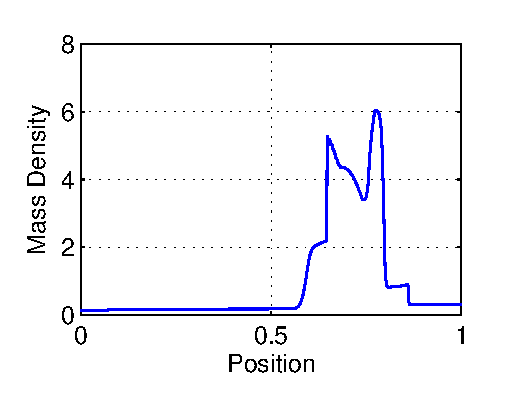
\includegraphics{DoubleBlast.eps}
\caption{Double Blast at t = 0.038}
\end{center}
\end{figure*}
\subsubsection{Initial Conditions}

Boundary conditions are mirrored around the X axis and periodic everywhere else.

The physical input parameters to the double blast test are:
\begin{itemize}
\item \tt{Pl} - Sets the pressure of the blastwave originating in the left-most tenth of the grid
\item \tt{Pr} - Similarly sets the pressure of the right-most blastwave
\item \tt{Pa} - Sets the ambient pressure
\end{itemize}


with the initial conditions set by each of the three zones being defined as an adiabatic gas with $\gamma$ = 1.4 everywhere. 
We set $\tt{Pl} = 1000$, $\tt{Pr} = 100$, and $\tt{Pa} = 0.01$. Initial momenta are zero everywhere.



\subsection{Einfeldt Strong Rarefaction Test}

This test measures the solver's vulnerability to very strong rarefactions that can, in some cases, 
produce negative mass densities or pressures. The input parameters can be tweaked slowly to determine 
exactly how strong the rarefaction can become before producing values that are NAN. 

\subsubsection{Analysis}

\subsubsection{Initial Conditions}

Einfeldt's Strong Rarefaction test consists of a 1-dimensional grid divided exactly in half. The 
properties of each half are defined separately, using four physical parameters. When run, the test 
produces two strong rarefaction waves moving away from the midpoint of the grid.

The physical input parameters to the Einfeldt Strong Rarefaction test are:
\begin{itemize}
\item \tt{rho} - Defines the mass density of the region
\item \tt{m} - Defines the X-momentum of the region (parallel to the grid)
\item \tt{n} - Defines the Y-momentum of the region (perpendicular to the grid)
\item \tt{e} - Defines the energy density of the region
\end{itemize}

The four parameters are saved separately as rhol and rhor, ml and mr, and so on.


\subsection{Hachisu (HSCF) Disk Simulation}

The Hachisu disk simulation generates a self-gravitating thick torus using the
method of Hachisu (1982) of solving the Poisson gravity equation simultaneously
with the q-parameterized rotation on cylinders model of a cylindrically symmetric gas disk.

This simulation is... not happy.

\subsubsection{Initial Conditions}

See Hachisu (1982) for derivation of equilibrium equations.

\subsubsection{Analysis}

...


\subsection{Implosion Symmetry Test}

The implosion symmetry test begins with initial conditions which have mirror symmetry
about the $x=y$ axis. Fluid mechanics dictates that then the exact solution will 
hold this symmetry forever.

Dimension-split codes are virtually never able to reproduce this condition forever
because their error commutators inevitably contain asymmetry-generating terms.

Because Imogen is dimensionally split, its error in this test is tracked by comparing
the ratio of the antisymmetric to symmetric components of the density.

\subsubsection{Initial Conditions}

Nominally any condition of mirror symmetry will do. The condition used by Athena consists of
a square domain of size 1x1, with
\begin{itemize}
\item $\rho(x+y < 1) = \rho_a$
\item $\rho(x+y \ge 1) = 1$
\item $P(x+y < 1) = P_a$
\item $P(x+y \ge 1) = 1$
\item $\vec{v} = 0$
\end{itemize}
By default the gas gamma is set to $7/5$ with $\rho_a = .125$ and $P_a = .14$.
All boundary conditions are mirrored.

The Imogen parameters are \begin{tt}Mcorner\end{tt} and \begin{tt}Pcorner\end{tt}.

This results in a standard Sod-like behavior in the middle of the corner/bulk region,
and a `jet' being launched along both edges, where the mirror boundary collides the two jets.
These jets promptly develop shear-flow instabilities. When they meet in the corner, they 
expel a two-lobed vortex down the $x=y$ line.

This is typically the point where the asymmetry component becomes obvious as this vortex is
intensely unstable to $x=y$-asymmetric disturbances.

\subsubsection{Analysis}




\subsection{Jet Test}

The jet test simulation initializes a uniform background, then sets up a fixed `injector' box
which fires fast-moving fluid into this background.

\subsubsection{Initial Conditions}

...

\subsubsection{Analysis}

Depending on the mach and the density of the injector fluid, several interesting behaviors are observable:
\begin{itemize}
\item Mach diamonds
\item KH instability: The jet always creates intense shearing motion, which results in KH turbulence at the jet/background boundary
\item RT instability: If the injector fluid is of low density, light fluid is accelerated into dense fluid and the ``bubble'' it blows out quickly deforms
\item Sound generation: A large simulation with long runtimes will be seen emitting sound waves into the far-field, away from the actual jet action
\end{itemize}



\subsection{Kelvin-Helmholtz Shearing Box Test}

The Kelvin-Helmholtz effect refers to the instability of a shearing surface to transverse structure formation.
It was first analyzed by Lord Kelvin (1871) and Hermann von Helmholtz (1868).

\subsubsection{Initial Conditions}

Imogen sets up the shearing motion in the X direction.

The initial conditions describe two regions of fluid at equal pressures, with opposite momenta
(such that the resulting structure is 'nominally stationary').

\subsubsection{Analysis}




\subsection{Radiative Hydrodynamic Shock Simulation}

Gasses subjected to a strong adiabatic shock will be heated very strongly. If the level of heating is sufficient,
the shocked fluid may be expected to radiate.

This creates an extended `shock' region consisting of the adiabatic jump, followed by a radiating region with
increasing density. Eventually a cutoff is reached, either physically (optical opacity) or numerically (temperature floor
in radiation function).

In the limit where the radiation time is taken to be extremely short compared to the flow time, the familiar
adiabatic Rankine-Hugoniot condition that $E_2 = E_1$ is replaced by the isothermal condition $T_2 = T_1$, resulting
in an isothermal shock.

\subsubsection{Initial Conditions}

The radiating shock simulation divides the X component of a 1-, 2- or 3-dimensional grid up into three
sections, the preshock, cooling, and cold gas layers.

Imogen accepts as input the parameters \begin{tt}fractionPreshock\end{tt} and \begin{tt}fractionCold\end{tt}.
The remainder forms the cooling region; Imogen chooses the grid spacing such that the distance from the shock
to the cold layer matches the length returned by the \begin{tt}RadiatingFlowSolver\end{tt} class.

This distance is approximately equal to the cooling length $L_{\text{cool}} \approx v_x \frac{\dot{P}}{P}$ which
in turn is defined by the shock's Mach number.

Imogen chooses frames such that the shock is initially stationary.

The \begin{tt}RadiatingFlowSolver\end{tt} class will generate a cooling region solution that is effectively exact, far
more accurate than the CFD code's truncation error.

Imogen requires an artificial parameter \begin{tt}Tcutoff\end{tt} which is the temperature that the cooling flow is allowed
to reach, in units of the preshock temperature. This value must be at LEAST one. In practice, it should be slightly
larger ($1.02-1.05$) to make both the shock jump discontinuity and the cold cutoff $\mathbb{C}^0$ points better behaved.

Without a temperature cutoff, a hydrodynamic radiating flow with a reasonable radiation law will cool to zero temperature,
infinite density and zero velocity in finite time and distance.

\subsubsection{Analysis}

...


\subsection{Rayleigh-Taylor Test}

The Rayleigh-Taylor test simulates a compressible form of the RT instability: lighter fluid which is
supporting (or being accelerated into) denser fluid is locally unstable.

In the inviscid case, any condition of pressure and density gradients pointing opposite ways will be
unstable in this manner.

\subsubsection{Initial Conditions}

Imogen sets up its RT simulation in a rectangular box, with circular conditions on X and Z and a fixed
potential field ('gravity') pulling in the -Y direction. The light/dense contact discontinuity is placed
at $Y = .5$. The parameters are
\begin{itemize}
\item \begin{tt}rhoTop\end{tt} - density of top fluid
\item \begin{tt}rhoBottom\end{tt} - density of lower fluid
\item \begin{tt}P0\end{tt} - the gas pressure at the BOTTOM of the column*
\item \begin{tt}pertAmplitude\end{tt} - the magitude of velocity perturbations
\item \begin{tt}Kx, Ky, Kz\end{tt} - wave vector for coherent perturbations
\item \begin{tt}randomPert\end{tt} - if true, uses random-per-cell velocities instead
\end{itemize}

\subsection{Analysis}

Lord Rayleigh's famous 1883 paper diagnosed the linear instability of the above described situation in the
incompressible case.

If the fluid is inviscid and the change of density is instant (contact discontinuity), the growth rate of
the linear instability in fact increases unboundedly with wavenumber and the system has \textit{zero} lifetime.

Viscosity, finite density gradient, and surface tension all establish short-wavelength cutoffs and regularize
the problem.




\subsection{Richtmyer-Meshkov Instability Test}

RMI occurs whenever a plane shockwave becomes incident upon a non-uniform density interface. 
The plane shock refracts through the interface, imparting differential vorticity that drives
a jet from the denser fluid into the lighter fluid.

\subsubsection{Analysis}

For this run, we used a square grid 2048 zones across, for 20,000 iterations.
\begin{figure*}
\begin{center}
\includegraphics[width=.5\textwidth]{RMI.eps}
\caption{Richtmyer-Meshkov instability at t = 6504}
\end{center}
\end{figure*}

\subsubsection{Initial Conditions}
Boundary conditions are periodic around the X axis, constant around the Y axis, and mirrored around the Z axis.

The physical input parameters to the Richtmyer-Meshkov Instability test are:
\begin{itemize}
\item \tt{mach} - Defines the mach speed of the incoming shock wave
\item \tt{rhotop} - Defines the density of the lighter fluid 
\item \tt{rhobottom} - Defines the density of the heavier fluid
\end{itemize}

To create the non-uniform interface, we create a cosine wave with an amplitude 1/20 of the height 
of the grid and with a wavelength 2x the length of the grid. We then place the center of the wave 
4 total wave amplitudes below the center of the grid, and set the mass density of the entire 
region below the wave equal to rhobottom. The rest of the grid is previously set to have density 
equal to rhotop, and is unchanged by the wave. We then create a shocked region from the top of 
the grid to a height just 20 zones above the peak of the wave. This shock is composed of a momentum 
and pressure equal to a blast wave with mach set by the input 'mach'.

Note that the entire region must then be given a momentum in the direction opposing the shock to 
maintain position on the grid. This opposing momentum is calculated by the same function as is used 
to calculate the initial shock.



\subsection{Sedov-Taylor Explosion Test}

The ST test measures the code's ability to capture high-Mach shocks and its ability to handle
them in multiple dimensions.

The initial conditions (analytically) for a Sedov-Taylor explosion consist of a spherically symmetric
fluid in N dimensions with
\begin{itemize}
\item $\rho(r) = \rho_0 r^-j$
\item $v(r) = 0$
\item $E_{\text{tot}}(r) = E / (\frac{4}{3} \pi \epsilon^3)$
\end{itemize}
In the standard classical ST case, $j=0$ and $N=3$ (producing a spherical explosion that models
the adiabatic phase of a nuclear explosion or supernova).


Details are in Sedov (1950), the best known of the original 3 ST papers. A modern derivation
which includes a walk-through explanation of the analysis and model code can be found in
Timmes 2000 \& Kamm \& Timmes (2002).

Under most conditions, the result is expected to maintain N-spherical symmetry.

KT also describe the existence of choices of physical ($j < N + 1$, resulting in finite mass within 
finite volume) solutions which have opposing pressure \& density gradients; These would be unstable 
to Rayleigh-Taylor induced convection.




\subsection{Sod Tube Test}

This test was used by Gary Sod in his 1976 paper that compared numerous then-in-use schemes
for 1D simulation of compressible supersonic dynamics.

While the original test parameters are no longer particularly challenging for any modern 
shock-capturing code, the Sod test is an enduring part of any test suite.

\subsubsection{Initial Conditions}

The Sod test refers to the solution of a particular Riemann problem:
\begin{itemize}
\item $\rho(x) = \{ 1, x < 0; .125, x \ge 0 \}$
\item $P(x) = \{ 1, x < 0; .1, x \ge 0 \} $
\item $\vec{v} = \vec{0}$
\end{itemize}
in an ideal gas with $\gamma = 7/5$.

Imogen uses a box of length 1, constant BCs, and runs to a time of 0.25.

\subsubsection{Analysis}

...




\subsection{Shu-Osher Tube Test}

Shu, C and Osher, S., "Efficient Implementation of Essentially Non-Oscillatory Shock-Capturing 
Schemes, II", J. Computational Physics, 83, 32-78 (1989). The test is Example 8. 

The grid is divided in half, with the left containing a shock and the right containing a sinusoidal 
structure in mass density. As the shock becomes incident upon the sinusoid, the structure of the 
sinusoid propogates out with the shockwave, translating and evolving but not acquiring any additional structure.

\subsubsection{Analysis}


\begin{figure*}
\begin{center}
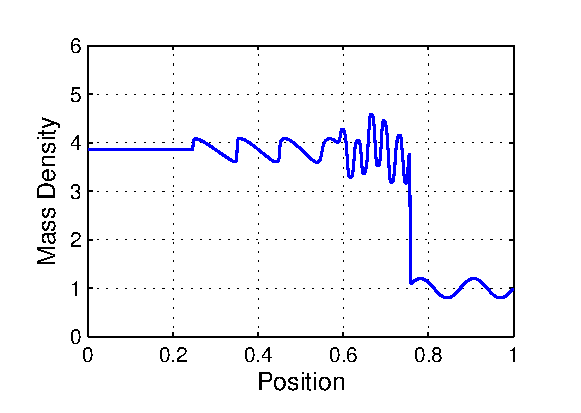
\includegraphics{ShuOsher.eps}
\caption{Shu-Osher Shocktube at t = 0.178}
\end{center}
\end{figure*}

\subsubsection{Initial Conditions}

Boundary conditions are constant around the X axis and periodic everywhere else.

The physical input parameters to the Shu-Osher test are:
\begin{itemize}
\item \tt{lambda} - Defines the wave number of the sinusoidal mass density structure
\item \tt{mach} - Defines the speed of the shockwave toward the sinusoid
\item \tt{waveAmplitude} - Defines the amplitude of the sinusoid
\end{itemize}




\end{document}
